This section documents the results obtained from the baseline as well as the experiments conducted using the importance features to train SVM classifier as describe in Section 3.9.
The reuslts of comparision of the performance of the final pipeline with the gold standard have also been documented here.

Table 4.1 shows the ROUGE scores obtained by comparing the baseline (TextRank) algorithm with the gold standard summaries.
It also shows the ROUGE scores of comapring the summaries generated by the final pipeline with the gold standard summaries.

\begin{table}[h]
\centering
\caption{ROUGE unigram scores}
\begin{tabular}{|l|l|l|ll}
\cline{1-3}
ROUGE (unigram) & TextRank & Final Pipeline &  &  \\ \cline{1-3}
Recall          & 0.447    & 0.536          &  &  \\ \cline{1-3}
Precision       & 0.452    & 0.466          &  &  \\ \cline{1-3}
F-measure       & 0.449    & 0.493          &  &  \\ \cline{1-3}
\end{tabular}
\end{table}

The classification results of using the importance features for training SVM are as follows.
\begin{itemize}
\item When I tried to train SVM classifier using tf-idf values, the model was extremly poor.
Even on the training set, the classifier was not able to classify any of the positive samples correctly.
\item Using count as the metric resulted in a similar model.
This time, not all positive samples were misclassified. But 90\% of the positive samples were misclassified.
Although, it is worth mentioning that the values of all the misclassified positive samples were close to 0.0 margin.
\item Using sec-tf-idf resulted in a better trained SVM model.
The precision and recall on the training set was 0.85 and .963 respectively.
The confusion matrix for the evaluation of this model over the test set is given in Table 4.2.
\begin{table}[h]
\centering
\caption{Confusion matrix for trained model using sec-tf-idf on test set}
\begin{tabular}{ll|c|c|}
                              &                                & \multicolumn{2}{c}{Predicted Class}                            \\ \cline{3-4} 
                              &                                & \multicolumn{1}{|l}{Positive} & \multicolumn{1}{|l|}{Negative} \\ \cline{2-4} 
\multirow{2}{*}{Actual Class} & \multicolumn{1}{|l|}{Positive} & 8                             & 25                             \\ \cline{2-4} 
                              & \multicolumn{1}{|l|}{Negative} & 3                             & 41                             \\ \cline{2-4} 
                              & \multicolumn{1}{|l}{Precision} & \multicolumn{2}{|c|}{72.73\%}                                  \\ \cline{2-4} 
                              & \multicolumn{1}{|l}{Recall}    & \multicolumn{2}{|c|}{24.24\%}                                  \\ \cline{2-4} 
\end{tabular}
\end{table}

The plots of the three features have been shown in Figure 4.1.
Here, 'red' represents positive samples and 'blue' represents negative samples.
The \textit{circle} represents correctly classified sentences and \textit{traingle} represents incorrectly classified sentences.

\begin{figure}[h]
\begin{subfigure}{0.5\textwidth}
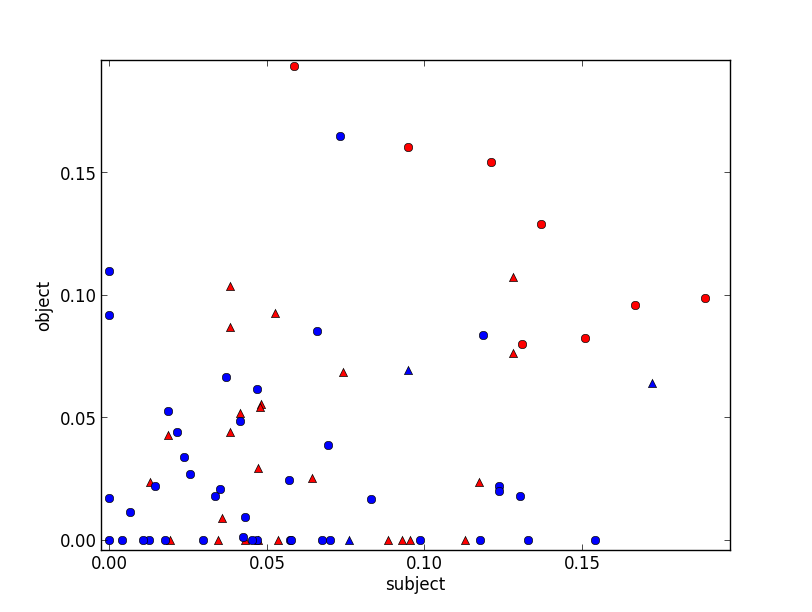
\includegraphics[width=0.9\linewidth, height=5cm]{obj-subj} 
\caption{Object - Subject Plot}
\label{fig:objsub}
\end{subfigure}
\begin{subfigure}{0.5\textwidth}
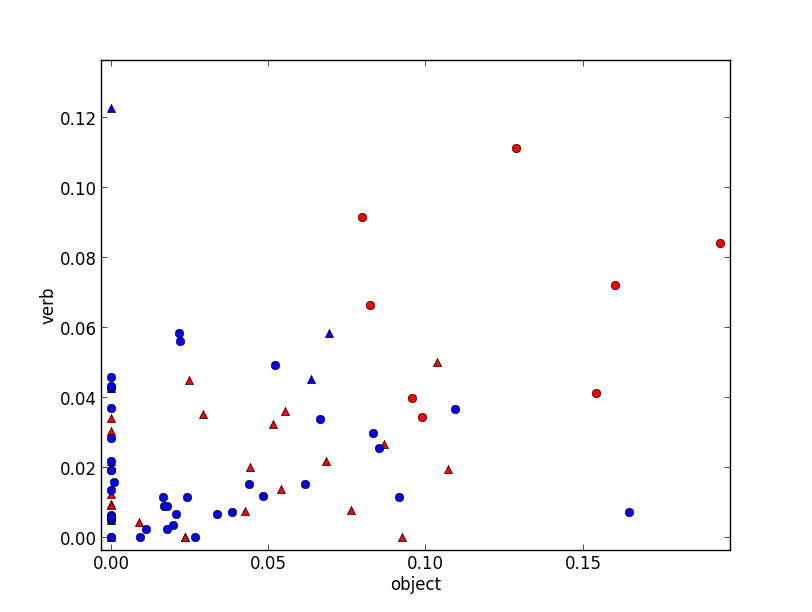
\includegraphics[width=0.9\linewidth, height=5cm]{verb-obj}
\caption{Verb - Object Plot}
\label{fig:verbobj}
\end{subfigure}
\begin{subfigure}{0.5\textwidth}
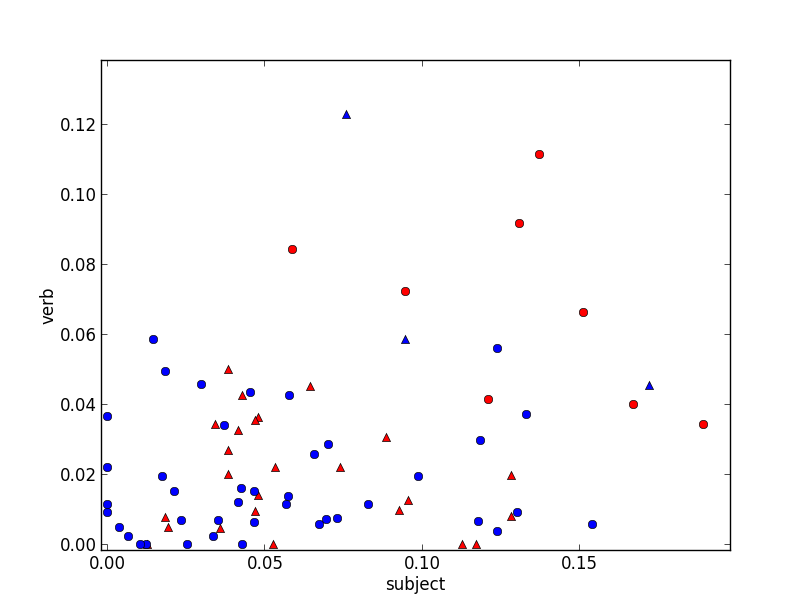
\includegraphics[width=0.9\linewidth, height=5cm]{verb-subj}
\caption{Verb - Subject Plot}
\label{fig:verbsubj}
\end{subfigure} 
\caption{Feature Plots}
\label{fig:feature-plots}
\end{figure}

\item The model trained using both count and sec-tf-idf values was as poor as the model trained using just the counts.
\item Varying the \textit{gamma} value for the RBF kernel did not show a drastic change in the overall performance of the classifier.
Table 4.3 shows the difference in the precision and recall on the test set as the gamma value was changed.
\begin{table}[h]
\centering
\caption{Change in Precision and Recall on the test set on varying gamma}
\begin{tabular}{|l|l|l|}
\hline
gamma & Precision & Recall \\ \hline
0.01  & 0.692     & 0.272  \\ \hline
0.1   & 0.692     & 0.272  \\ \hline
1.0   & 0.692     & 0.272  \\ \hline
10    & 0.81      & 0.27   \\ \hline
100   & 0.81      & 0.27   \\ \hline
\end{tabular}
\end{table}
\item Varying the decaying factor for calculation of sec-tf-idf value did not show any drastic change in the performance.
Table 4.4 shows the values of precision and recall on the test set as the decaying factor is changed.
\begin{table}[h]
\centering
\caption{Change in Precision and Recall on varying the decay factor}
\begin{tabular}{|l|l|l|}
\hline
Decay & Precision & Recall \\ \hline
0.2   & 0.777     & 0.212  \\ \hline
0.5   & 0.8       & 0.24   \\ \hline
1.0   & 0.692     & 0.272  \\ \hline
1.5   & 0.769     & 0.303  \\ \hline
\end{tabular}
\end{table}
\end{itemize}

Although the test set was small in size, the sentences in this set were manually labelled unlike the sentences in the training set whose lables were approximated.
So in order to validate the performance of this model, I dediced to use the test set for k-fold validation.
The results of such validation can be extrapolated to estimate the performance of this model over a larger data set.
With 11 sentences in each set, I conducted a 7-fold validation.
The average values of precision was 0.81 and recall was 0.35.
This is slightly better than the performance of the  model over the entire test set and can be attributed to the small size of the data set.
However, this also shows that the validation result was close to the test set evaluation and hence the model is expected to perform similarly with larger training and test sets.